\subsection{Minimap creation}
To create the minimap are needed:
\begin{itemize}
	\item An image that contains an empty billiard table and some information about it;
	\item The position of the balls in the current and previous frames;
	\item A transformation matrix that computes the position of the balls in the minimap.
\end{itemize}

\subsubsection{Empty minimap image}
As a first step, an image of an empty billiard table has been selected, and its corner positions and dimensions have been stored in constant variables by testing different values. In particular Alberto had the idea of converting the image into a byte array and inserting it in a header file through ImageMagick (\url{https://imagemagick.org/}).
This step has been performed with the aim of creating a self-contained executable without the need of the png image dependency.
The byte array is then used to create a \texttt{Mat} object through the \texttt{imdecode} function.

\subsubsection{Computation of the transformation matrix}
The \texttt{computeTransformation} method has been written to compute the transformation matrix, which allows for the computation of the positions of the balls in the 2d table represented in the minimap. To do that, a relationship between the corners of the table in the frame and the corners of the table in the minimap has been found by the OpenCV \texttt{getPerspectiveTransform()} method, which “calculates a perspective transform from 4 pairs of the corresponding points” and returns a transformation matrix.
At first, it is supposed that the corners are given in clockwise order and that the first corner is followed by a long table edge. To check this information, \texttt{checkHorizontalTable} has been written.

\subsubsection{Check if the corners are in the required order}	% TODO pool -> pocket
The \texttt{checkHorizontalTable} method checks, using the image in input and the corners of the table in that image, if the corners are oriented such that the first corner is followed by a long table edge.
To check this information, the “percentage of table” with respect to the pool in a rectangle placed in the center of the edge (with dimensions proportional to the real table and pool dimensions) has been computed for all the edges. This computation has been done in the table image previously transformed and cropped to the table dimensions; in this way, the center between two corners corresponds to the real one (otherwise, if the table has some perspective effect, the center between the two corners may not correspond to the real one). Then, the edges have been ordered by using this percentile. To understand how the corners were oriented, three cases have been considered:
\begin{itemize}
	\item If the edges with "more pool" are opposite edges, then they are the longest edges; This happens, for example, in Figure \ref{fig:game2_clip1_orientation}.
	\item If the edge with "more pool" is opposite to the one with "less pool", then they are not the longest edges; This happen, for example, in Figure \ref{fig:game3_clip1_orientation} and Figure \ref{fig:game4_clip1_orientation}, when there is an occlusion or much noise in the center of the edge with "more pool".
	\item Otherwise, there is uncertainty, and then, probably, the one with "more pool" is the longest edge.
\end{itemize}
If the table is not horizontal as expected (for example in Figure \ref{fig:game1_clip1_orientation}), then all the edges are rotated and the transformation matrix is re-computed.

\begin{figure}[H]
	\centering
	\begin{subfigure}[b]{0.48\textwidth}
		\centering
		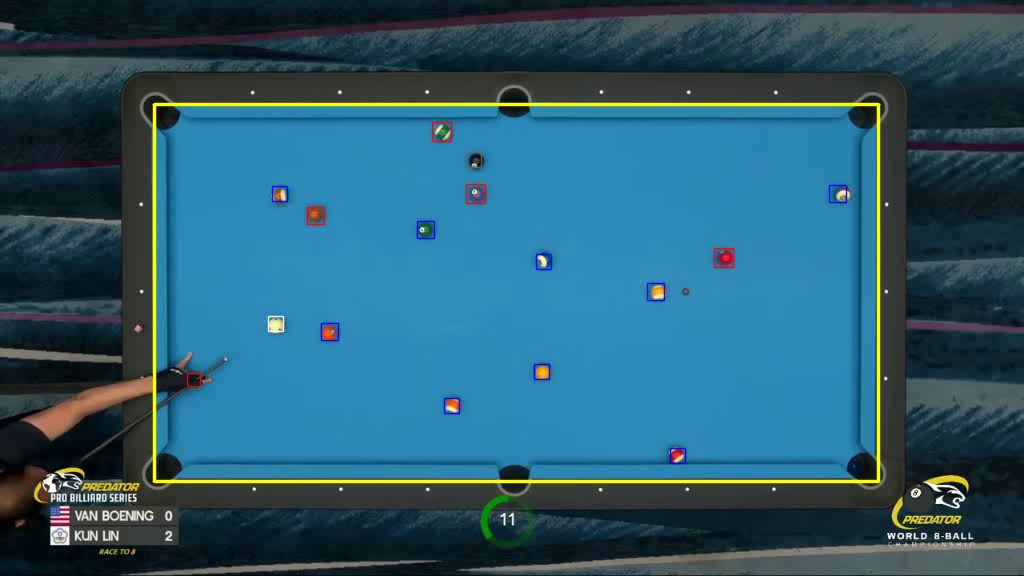
\includegraphics[width=\textwidth]{images/TableOrientation/g1_c1.jpg}
		\caption{Detection of the table and the balls with the colors representing the classes.}
		%\label{fig:game1_clip1_detection}
	\end{subfigure}
	\begin{subfigure}[b]{0.48\textwidth}
		\centering
		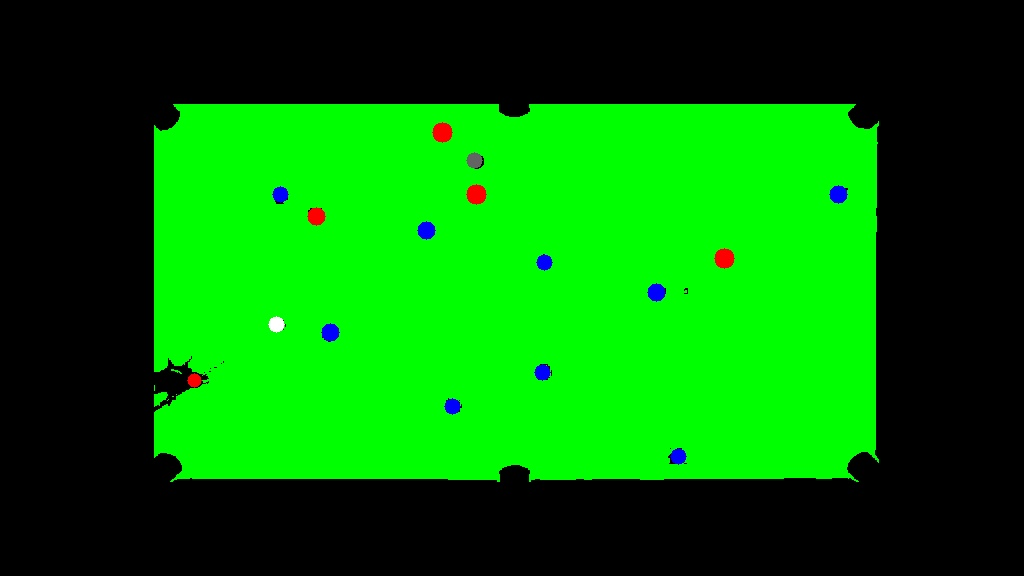
\includegraphics[width=\textwidth]{images/Segmentation/game1_clip1_segmented_balls_first_frame.jpg}
		\caption{Transformation of the table to the minimap table size}
		%\label{fig:game1_clip1_mask}
	\end{subfigure}
	\caption{game1\_clip1 first frame. The table is transformed in a wrong way, because the pools are located in the shortest edges rather than the longest ones.}
	\label{fig:game1_clip1_orientation}
\end{figure}

\begin{figure}[H]
	\centering
	\subfloat[Detection of the table and the balls with the colors representing the classes.]{
		%\label{fig:game2_clip1_detection}
		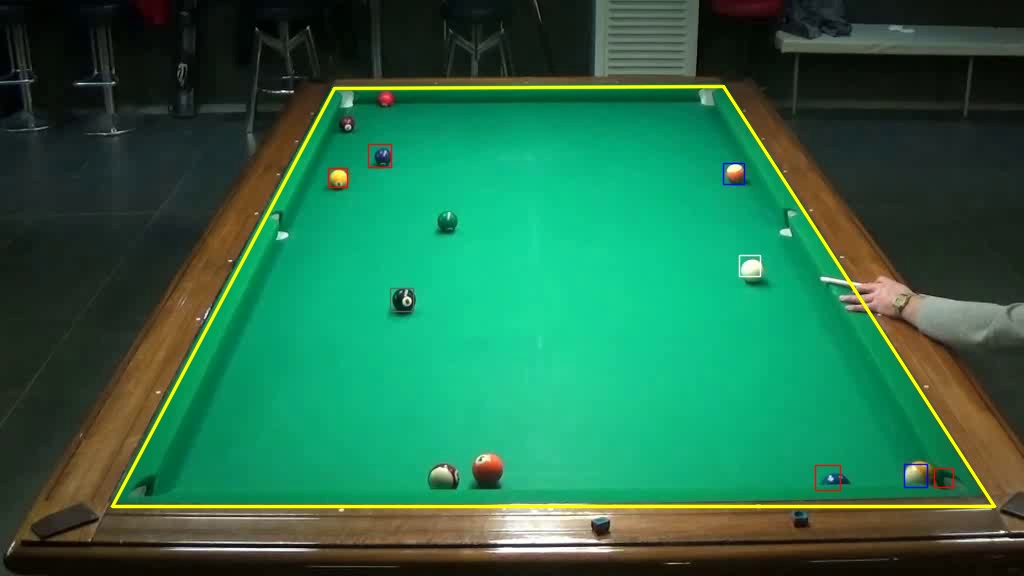
\includegraphics[width=0.48\textwidth]{images/TableOrientation/g2_c1.jpg}
	}
	\
	\subfloat[Transformation of the table to the minimap table size.]{
		%\label{fig:game2_clip1_mask}
		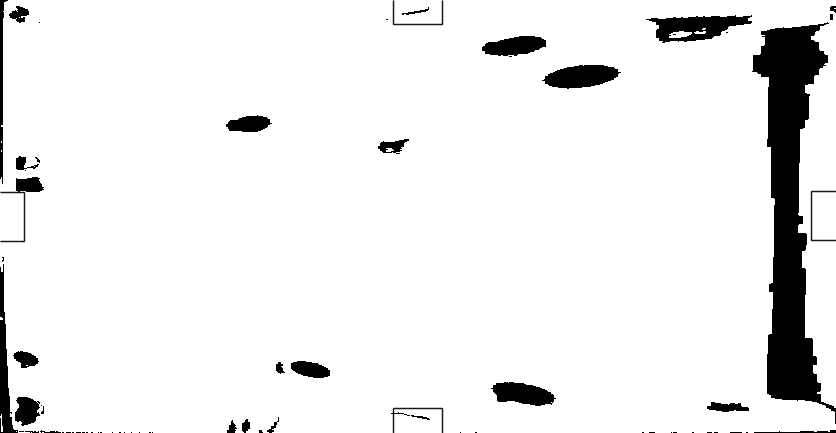
\includegraphics[width=0.48\textwidth]{images/TableOrientation/g2_c1_mask.jpg}
	}
	\caption{game2\_clip1 first frame. The table is correctly transformed. In this case the pools are lightly visible, but they allow to detect the correct orientation.}
	\label{fig:game2_clip1_orientation}
\end{figure}

\begin{figure}[H]
	\centering
	\subfloat[Detection of the table and the balls with the colors representing the classes.]{
		%\label{fig:game3_clip1_detection}
		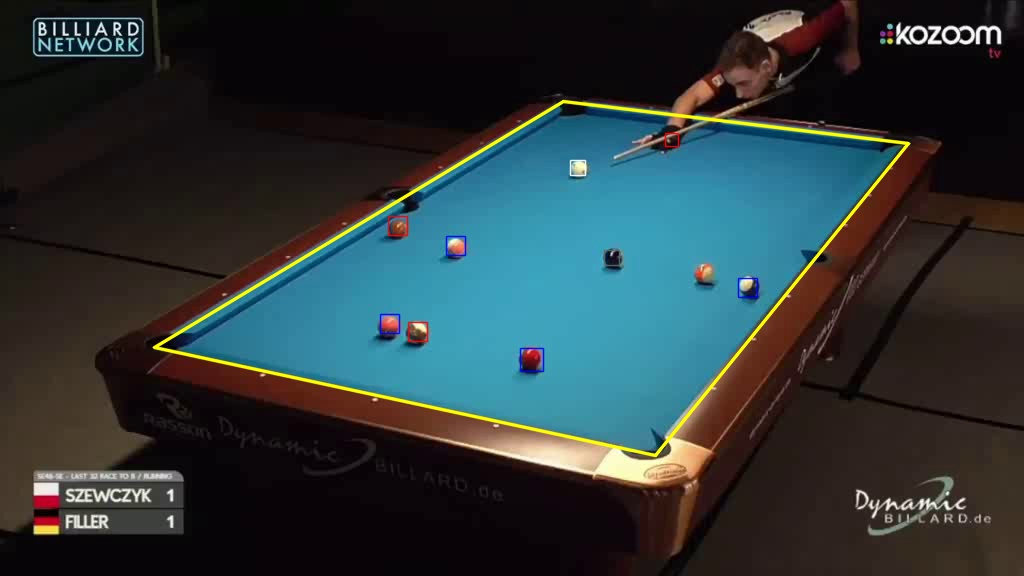
\includegraphics[width=0.48\textwidth]{images/TableOrientation/g3_c1.jpg}
	}
	\
	\subfloat[Transformation of the table to the minimap table size.]{
		%\label{fig:game3_clip1_mask}
		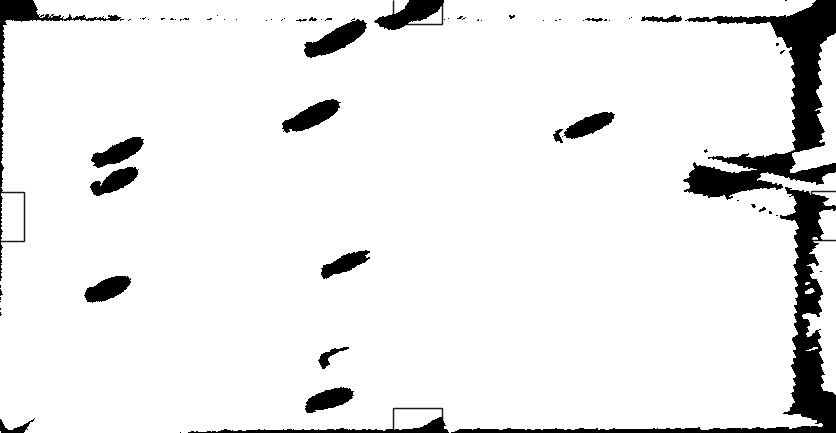
\includegraphics[width=0.48\textwidth]{images/TableOrientation/g3_c1_mask.jpg}
	}
	\caption{game3\_clip1 first frame. The table is correctly transformed. In this case, the center of one of the shortest edges has some noise due to the person playing the game; the result is correct, because in the opposite edge there is no noise.}
	\label{fig:game3_clip1_orientation}
\end{figure}

\begin{figure}[H]
	\centering
	\subfloat[Detection of the table and the balls with the colors representing the classes.]{
		%\label{fig:game4_clip1_detection}
		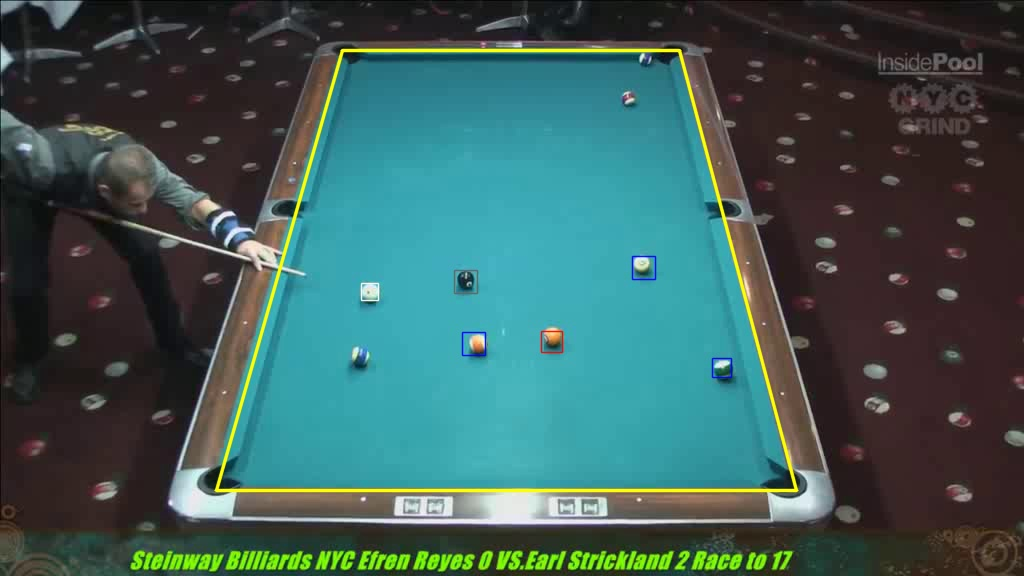
\includegraphics[width=0.48\textwidth]{images/TableOrientation/g4_c1.jpg}
	}
	\
	\subfloat[Transformation of the table to the minimap table size.]{
		%\label{fig:game4_clip1_mask}
		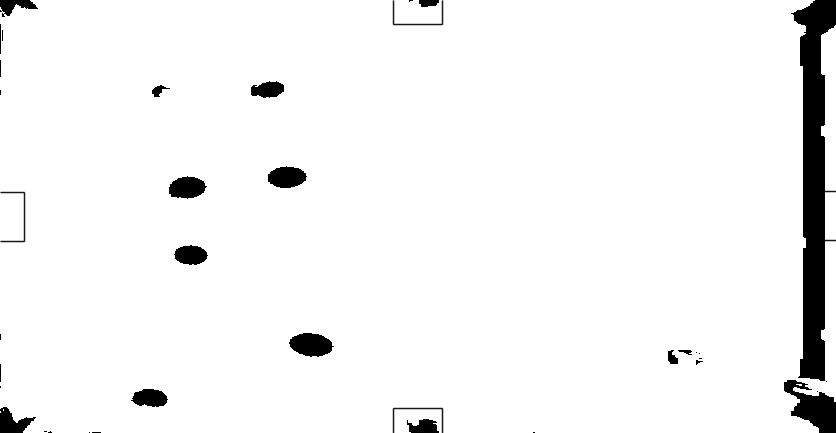
\includegraphics[width=0.48\textwidth]{images/TableOrientation/g4_c1_mask.jpg}
	}
	\caption{game4\_clip1 first frame. The table is correctly transformed. In this case, the center of one of the shortest edges has some noise due to the light of the table; the result is correct, because in the opposite edge there is no noise.}
	\label{fig:game4_clip1_orientation}
\end{figure}


\subsubsection{Draw the minimap with tracking lines and balls}
Given the transformation matrix and the ball positions in the frame, it is possible to compute the positions of the balls in the minimap. This computation has been done in the \texttt{drawMinimap} method. Every time this method is called, the ball positions and the positions of the balls in the previous frame (if they have been computed by the tracker) are computed by using the \texttt{perspectiveTransform} method. For each ball in the frame, a line between the previous position and the current position is drawn on the minimap image, passed as a parameter by reference such that all the tracking lines are kept in a single image (Figure \ref{fig:game2_clip1_tracking}). Then this image is cloned into a copy, and the current balls are drawn on it. This image is then returned (Figure \ref{fig:game2_clip1_balls}). This implementation idea comes from Alberto.

\begin{figure}[H]
	\centering
	\begin{subfigure}[b]{0.48\textwidth}
		\centering
		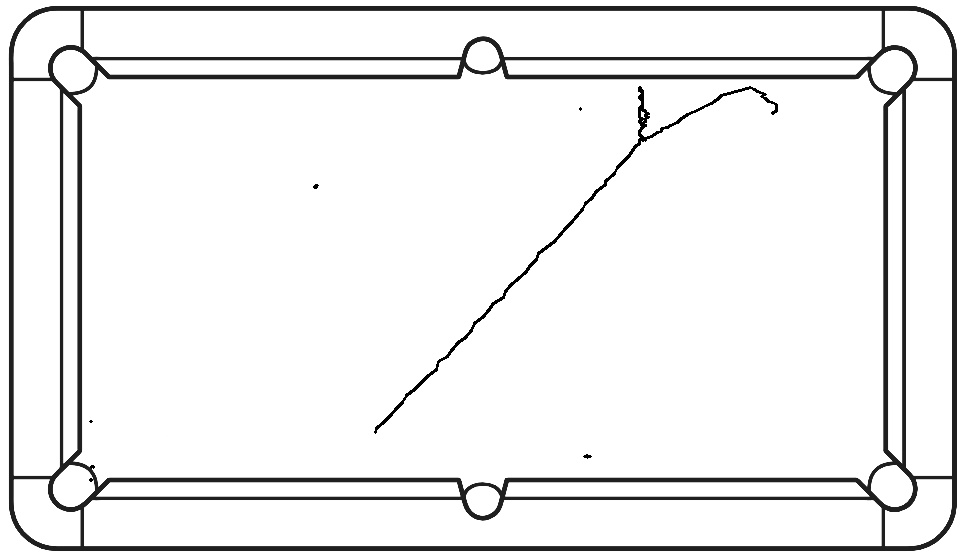
\includegraphics[width=\textwidth]{images/Minimap/g2_c1minimap_with_track.jpg}
		\caption{Minimap with tracking lines}
		\label{fig:game2_clip1_tracking}
	\end{subfigure}
	\begin{subfigure}[b]{0.48\textwidth}
		\centering
		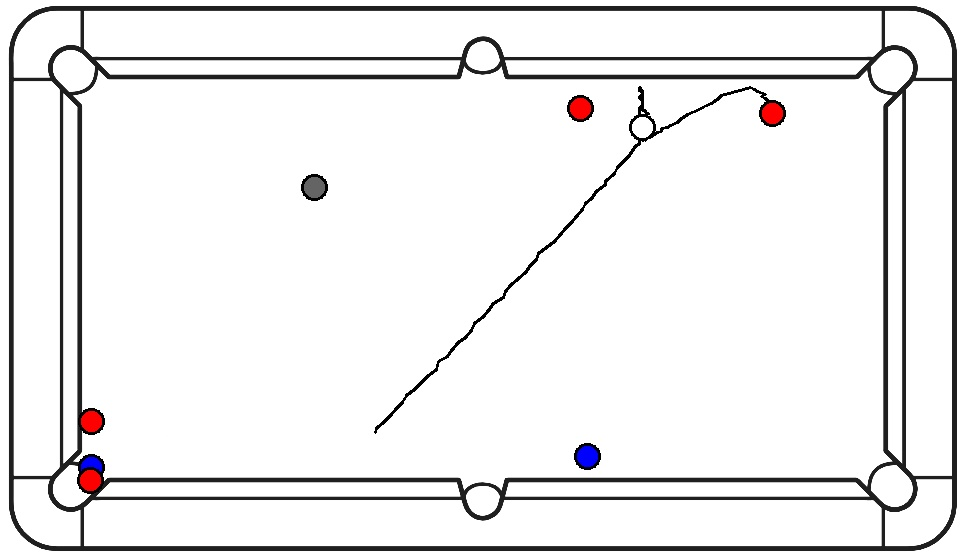
\includegraphics[width=\textwidth]{images/Minimap/g2_c1_minimap_with_balls.jpg}
		\caption{Minimap with tracking lines and balls}
		\label{fig:game2_clip1_balls}
	\end{subfigure}
	\caption{game2\_clip1. Minimap of the last frame.}
	\label{fig:game2_clip1_balls_and_tracking}
\end{figure}

The ideas of using and the implementation of \texttt{getPerspectiveTransform} and \texttt{perspectiveTransform}, and how to check the orientation of the table were from Michela.
